\glsreset{clf}\glsreset{cbf}
This chapter lays the basics of all shared control theory applied in the following chapters dealing with the design of a safe controller.

Based on \citep{bib:artstein}, who founded \glspl{clf} based on Lyapunov functions described in \autoref{eq:lyap}, a \gls{cbf} can be created according to \citep{bib:org_control} from where the definition below is stated:
\begin{defn}[Control Barrier Function]\label{def:cbf}
Given a system $\dot{\mathbf{x}}=f(\mathbf{x})+g(\mathbf{x})\mathbf{u}$, the function $B:\mathbb{R}^n\rightarrow\mathbb{R}$ is a \gls{cbf} if the below constraints are fulfilled:
\begin{subequations}\label{eq:reqs}
\begin{flalign}
\mathbf{x}\in \mathcal{X}_u \hspace{0.3cm} &\Rightarrow \hspace{0.3cm} B(\mathbf{x}) > 0  \label{req1} \\
L_gB(\mathbf{x}) = 0 \hspace{0.3cm} &\Rightarrow \hspace{0.3cm} L_fB(\mathbf{x}) < 0 \label{req2} \\
\{ \mathbf{x} \in \mathcal{X} \,\,|\,\, B(\mathbf{x}) \leq 0 \} &\neq \emptyset \label{req3}
\end{flalign}
\begin{tabular}{r  l} 
where  &  \\
$B(\mathbf{x})$ & is a control barrier function  \\ 
$L_fB(\mathbf{x})$ & is the Lie derivative of $B(\mathbf{x})$ along the vector field  $f(\mathbf{x})$, i.e. $\frac{d B(\mathbf{x})}{d \mathbf{x}}f(\mathbf{x})$  \\ 
$L_gB(\mathbf{x})$ & is the Lie derivative of $B(\mathbf{x})$ along the vector field  $g(\mathbf{x})$, i.e. $\frac{d B(\mathbf{x})}{d \mathbf{x}}g(\mathbf{x})$ \\
\end{tabular}\\

The requirement in \autoref{req2} can be hard to fulfill, and can be replaced with a relaxed constraint to obtain a weak \gls{cbf}:
\begin{equation}
L_gB(\mathbf{x}) = 0 \hspace{0.3cm} \Rightarrow \hspace{0.3cm} L_fB(\mathbf{x}) \leq 0 \label{req2_weak}
\end{equation}
\end{subequations}
\end{defn}
Note how \autoref{def:cbf} put forth demands for the open loop system as opposed to \autoref{def:barrier_certificate}	which describes the closed loop system. \Autoref{req1}  essentially states the same as \autoref{cer2}, i.e. when $B(\mathbf{x})>0$ then \textbf{x} is in the unsafe region. This makes it possible to design both the unsafe and the safe region by shaping $B(\mathbf{x})$. \Autoref{req2} puts forth the requirement that the gradient along the vector field $f(\mathbf{x})$ must point away from the unsafe area, bounded by the zero level set of the barrier function, whenever the state cannot be controlled by the input (except in the critical point as the system is in its equilibrium at this point). \Autoref{req3} simply states that the safe area must contain some states as control otherwise is impossible.
%
\section{The Control Law}\label{eq:control_for_safety}
It is convenient to divide the control law into two controllers. A controller that is used in an area close to the unsafe region and a controller used in the safe region. The reason for this divided control law is the ability to apply linear control theory in the safe area  (the system can be well approximated as a linear second order system, see \autoref{sec:model_slide}) and thereby make use of the benefits from linear control.
 %he old Chinese proverb, \textit{"Do not use a cannon to kill a mosquito"}, thus why not use a simple controller in the safe region
Thus the safe set $\mathcal{X}_0$ is divided into two sections: a transition space $\mathcal{T}$ being the subset of the safe region closest to the unsafe set where safety control should be applied, and the remaining safe region  $\mathcal{Y}$ where linear control can be applied, thus introducing a divided control law:
\begin{flalign}
u(\mathbf{x}) =
\begin{cases}
	\tilde{u}(\mathbf{x}) \kk &\text{if} \mm \mathbf{x} \in \,\, \text{\gls{Yfancy}}\subset\mathcal{X}_0 \\
	 k_0(\mathbf{x})  \kk &\text{if} \mm \mathbf{x} \in \,\, \text{\gls{Tfancy}}= \mathcal{X}_0\setminus\mathcal{Y}
\end{cases}\label{eq:u_utilde_k0}
\end{flalign}
\begin{tabular}{rp{14cm}} 
where  &  \\
\gls{u_tilde} & is the non-safe controller applied on $\mathcal{Y}$ well within the safe region, $\tilde{u}(\mathbf{x}) \in \mathbb{R}^m$\\
\gls{k0} & is a controller guaranteeing system safety, applied in the transition space $\mathcal{T}$ close to the unsafe set, $k_0(\mathbf{x}) \in \mathbb{R}^m$\\
\end{tabular}\\

%The controller $\tilde{u}(\mathbf{x})$ used for $\mathbf{x} \in \mathcal{Y}$ will be referred to as a non-safe controller and the controller $k_0(\mathbf{x})$ used for $\mathbf{x} \in \mathcal{T}$ will be referred to as a safety controller or a controller ensuring safety. 
For a linear system, the non-safe controller can be determined by linear state feedback:
\begin{flalign}
\tilde{u}(\mathbf{x}) = \bar{\mathbf{N}}\,\mathbf{x}_\text{ref} - \mathbf{K}\,\mathbf{x}
\label{eq:utilde}
\end{flalign}
\begin{tabular}{rl} 
where  &  \\
$\mathbf{K}$ & is a constant feedback matrix for a system with $n$ states and $m$ inputs, $\mathbf{K} \in \mathbb{R}^{m \times n}$ \\
$\bar{\mathbf{N}}$ & is a constant to ensure unity gain from reference to output, $\bar{\mathbf{N}} \in \mathbb{R}^{m\times m}$ \\
$\mathbf{x}_\text{ref}$ & is the position reference, $\mathbf{x}_\text{ref} \in \mathbb{R}^m$ \\
$\mathbf{x}$ & is the state vector, $\mathbf{x} \in \mathbb{R}^{n}$\\
\end{tabular}\\

The two controllers can be combined as a linear combination determined by a parameter \gls{sigma}$\in[0,1]$ \citep{bib:org_control}. This ensures that the switch between the two controllers occurs with less fluctuations. 
\begin{flalign}
u(\mathbf{x},\tilde{u}) &= \sigma(\mathbf{x})k_0(\mathbf{x})+(1-\sigma(\mathbf{x}))\tilde{u}(\mathbf{x}) \label{eq:control_law}
% &= \sigma(x)k_0(x)+(1-\sigma(x))(\bar{N} \cdot x_\text{ref}-Kx) \label{eq:control_law}
\end{flalign}
%\begin{tabular}{rp{13.7cm}} 
%where  & \\
%%$u(x) \in \mathbb{R}^{m \times 1} $is a control signal where safety is ensured  & [$\cdot$] \\
%%$\tilde{u}(x) \in \mathbb{R}^{m \times 1}$ is a control signal to the linear state space system such that $\tilde{u}=\bar{N}\cdot x_\text{ref}-Kx $ & [$\cdot$] \\ 
%$k_0(\mathbf{x})$ & is a control law that guarantees safety, $k_0(\mathbf{x}) \in \mathbb{R}^m$  \\ 
%$\sigma(x)$ & %such that $0 \leq \sigma(x) \leq 1$, 
%founds a linear combination between the two controllers, $\sigma(x) \in [0,1]$ \\ 
%%$K \in \mathbb{R}^{m \times n}$ is a constant feedback matrix where $n$ is the number of states & [$\cdot$] \\
%%$\bar{N} \in \mathbb{R}^{m \times 1}$ is a constant to ensure unity gain from reference to output & [$\cdot$] \\
%%$x \in \mathbb{R}^{n \times 1}$ is the state vector& [$\cdot$] 
%\end{tabular}\\

Note the two extremities of  $\sigma(\mathbf{x})$:
\begin{flalign*}
\sigma(\mathbf{x}) = 
\begin{cases}
0 \mm &\Rightarrow \mm \text{Pure control by pole placement, i.e. $u(\mathbf{x}) = \tilde{u}(\mathbf{x}) =  \bar{\mathbf{N}} \mathbf{x}_\text{ref}-\textbf{Kx}$ } \\
1 \mm &\Rightarrow \mm \text{Pure safety control i.e. $u(\mathbf{x}) = k_0(\mathbf{x})$ }
\end{cases}
\end{flalign*}
The interval between 0 and 1 can be refined such that the transition between the two control laws is not instantaneous. This smoothing can be performed with a smooth approximation of the unit step (a bump function) of $B(\mathbf{x})$ by introducing a scalar \gls{epsilon} $>0$ \citep{bib:org_control}:
\begin{flalign}
\sigma(\mathbf{x}) = 
\begin{cases}
0 & \text{if} \mm B(\mathbf{x}) \leq -\epsilon \\
-2  \left( \dfrac{B(\mathbf{x})}{\epsilon} \right)^3 - 3\left( \dfrac{B(\mathbf{x})}{\epsilon} \right)^2 +1 \kk &\text{if} \mm B(\mathbf{x}) \in (-\epsilon,0) \\
1  &\text{if} \mm B(\mathbf{x}) \geq 0
\end{cases}
\label{eq:smoothness}
\end{flalign} 
%
%
% 
A block diagram of a linear closed loop system with control input as described in \autoref{eq:control_law} is depicted in \autoref{fig:controlsystem}.
\begin{figure}[h]
\centering
	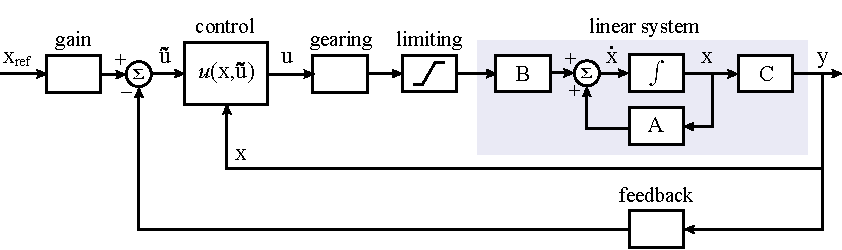
\includegraphics[width=\textwidth]{control_system.pdf}
	\caption{Block diagram of the control system. The limiter limits the control signal such that it does not exceed the physical boundaries of the da Vinci robot. The gearing ensures that there is a 1:1 mapping between the control signal and the physical position, i.e. meters for prismatic joints and radians for revolute joints.}
	\label{fig:controlsystem}
\end{figure}

\subsection{Uniform Construction of the Safety Controller $k_0$(x)}
The control law ensuring safety can be found as \citep{bib:org_control}:
\begin{flalign}
k_0(\mathbf{x}) = \begin{cases}
-\dfrac{L_fB(\mathbf{x})+ \sqrt{(L_fB(\mathbf{x}))^2 + \kappa^2L_gB(\mathbf{x})(L_gB(\mathbf{x}))^T}}{L_gB(\mathbf{x})(L_gB(\mathbf{x}))^T}(L_gB(\mathbf{x}))^T &\text{if} \mm L_gB(\mathbf{x}) \neq 0 \\
0  &\text{if} \mm L_gB(\mathbf{x}) = 0
\end{cases}
\label{eq:control_law_safety}
\end{flalign}
where $\kappa$ is a design variable. High values of $\kappa$ implies increased controller aggressiveness. \Autoref{eq:control_law_safety} indeed ensures safety for the closed loop system $\dot{\mathbf{x}} = f(\mathbf{x})+g(\mathbf{x})k_0(\mathbf{x})$. This is easily proven as:
\begin{flalign*}
L_{f_{cl}}B(\mathbf{x}) = L_fB(\mathbf{x}) + L_gB(x)k_0(\mathbf{x})
\end{flalign*}
For $L_gB(\mathbf{x}) \neq 0:$
\begin{flalign*}
L_{f_{cl}}B(\mathbf{x}) &= L_fB(\mathbf{x}) + L_gB(\mathbf{x}) \left( -\dfrac{L_fB(\mathbf{x})+ \sqrt{(L_fB(\mathbf{x}))^2 + \kappa^2L_gB(\mathbf{x})(L_gB(\mathbf{x}))^T}}{L_gB(\mathbf{x})(L_gB(\mathbf{x}))^T}(L_gB(\mathbf{x}))^T \right)  \\
&= L_fB(\mathbf{x}) - L_gB(\mathbf{x})(L_gB(\mathbf{x}))^T \dfrac{L_fB(\mathbf{x}) + \sqrt{(L_fB(\mathbf{x}))^2 + \kappa^2L_gB(\mathbf{x})(L_gB(\mathbf{x}))^T}}{L_gB(\mathbf{x})(L_gB(\mathbf{x}))^T}   \\ 
&= L_fB(\mathbf{x}) - L_fB(\mathbf{x}) - \sqrt{(L_fB(\mathbf{x}))^2 + \kappa^2L_gB(\mathbf{x})(L_gB(\mathbf{x}))^T} \\
&= - \sqrt{(L_fB(\mathbf{x}))^2 + \kappa^2 L_gB(\mathbf{x})(L_gB(\mathbf{x}))^T} \mm \leq 0 \mm \forall \mm \mathbf{x}
\end{flalign*}
As all terms within the square root are squared, no imaginary numbers occur, and as a result $L_{f_{cl}}B(\mathbf{x})$ will always be nonpositive when $L_gB(\mathbf{x}) \neq 0$.
According to \autoref{eq:control_law_safety}, when $L_gB(\mathbf{x}) = 0$:
\begin{flalign*}
L_{f_{cl}}B(\mathbf{x}) = L_fB(\mathbf{x}) + L_gB(\mathbf{x})\cdot 0 = L_fB(\mathbf{x})
\end{flalign*}
As $B(\mathbf{x})$ is constructed such that whenever $L_gB(\mathbf{x}) = 0$ then it is always true that $L_fB(\mathbf{x}) < 0$, it is thereby verified that $Lf_{cl}B(\mathbf{x})\leq 0$ for all $\mathbf{x} \in\mathcal{X}$. 

\section{Using CBFs in the Control Design for the da Vinci Robot}
The theory presented in this chapter allows a way to construct a controller such that safety is guaranteed, if the constraints on the \gls{cbf} in \autoref{def:cbf} are obeyed.
%\textcolor{red}{This is true but there is a place where we change from one to the other system, where we in principle do not know what happens. [RAFAEL]}
It may, however, be noted that when the controller is transferred to a digital system, the certificate is built upon an infinite sampling rate as the certificates are described in continuous time. Adopting the certificate to a discrete system is indeed a challenge worth respecting. 

%\textcolor{red}{And now, how do you use this.What do you use the reference for etc. Remember to shape the thing according to your problem also. Also have in mind that these concepts are NOT standard knowledge by control engineers. Therefore, they should be thoroughly introduced. [CHRISTOFFER]}

\glspl{cbf} will be used in the following chapters to design safe controllers for the da Vinci surgical robot. In \autoref{chap:cbf_1d_static} a controller is designed that ensures safety for the slide movement of the robot (sliding the tool up and down in one dimension, see \autoref{fig:naming_convention})  thereby illustrating the usefulness of the theory. In \autoref{chap:cbf_1d_dynamic} the theory is used to establish the basics for surgery on a beating heart and in  \autoref{chap:cbf_3d_static} the system is  expanded to 3D Cartesian space including all the controllable joints of the robot. For the ROS implementation of the controllers, the reader is referred to appendix \ref{appsec:ros_development}.



